\chapter{IQ twist}
\section{CSP model}
\newcommand{\VUnits} {\ensuremath{V_{units}}}
\newcommand{\VPegs} {\ensuremath{V_{pegs}}}
\newcommand{\Constraints}[2] {\ensuremath{C_{v_{#1},v_{#2}}}}
\newcommand{\Cons}[5] {\ensuremath{C_{v_{#1},v_{#2},v_{#3},v_{#4},v_{#5}}}}
\newcommand{\Con}[3] {\ensuremath{C_{v_{#1},v_{#2},v_{#3}}}}
\newcommand{\Const}[4] {\ensuremath{C_{v_{#1},v_{#2},v_{#3},v_{#4}}}}
\newcommand{\Constraint}[1] {\ensuremath{C_{v_{#1}}}}
\newcommand{\Domain}[1] {\ensuremath{D(v_{#1})}}
\label{sec:CSP model}
In this part, I'd like to use CSP to model the IQ twist game. Above all, I'd like to define all the initial state for each piece:
\begin{center}

\includegraphics{yellow1.jpg} 
\\initial state of Yellow 1
\\
\includegraphics{yellow2.jpg}
\\initial state of Yellow 2
\\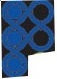
\includegraphics{blue1.jpg}
\\initial state of Blue 1
\\
\includegraphics{blue2.jpg}
\\initial state of Blue 2
\\
\includegraphics{green1.jpg}
\\initial state of Green 1 
\\
\includegraphics{green2.jpg}
\\initial state of Green 2
\\
\includegraphics{red1.jpg}
\\initial state of Red 1 
\\
\includegraphics{red2.jpg}
\\initial state of Red 2 
\end{center}
For this method, there are some rules. Firstly, all the variables correspond to the initial states. Such as the Yellow 2, I use $V_{y21}$ to represent the left and bottom unit. For other variables, name them as $V_{y22}$, $V_{y23}$, $V_{y24}$ and $V_{y25}$ follow the order from left to right and bottom-up.
\begin{center}
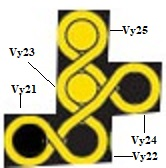
\includegraphics{example.jpg}
\\naming rules example for yellow 2
\end{center}
For the board, I use the rectangular coordinate system to represent positions. 
\begin{center}
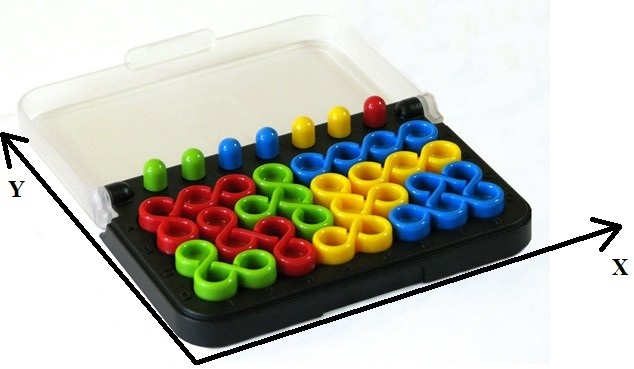
\includegraphics{IQtwistboard.jpg}
\\method of represent positions
\end{center}
\subsection{Variables}
\begin{align*}
\VUnits=\{&V_{y11},V_{y12},V_{y13},\\&V_{y21},V_{y22},V_{y23},V_{y24},V_{y25},\\&V_{b11},V_{b12},V_{b13},V_{b14},
V_{b15},\\&V_{b21},V_{b22},V_{b23},V_{b24},\\&V_{g11},V_{g12},V_{g13},V_{g14},\\&V_{g21},V_{g22},V_{g23},\\&V_{r11},
V_{r12},V_{r13},V_{r14},\\&V_{r21},V_{r22},V_{r23},V_{r24}\}\\
\\\VPegs = \{&V_{py1}, V_{py2}, V_{pb1}, V_{pb2}, V_{pg1}, V_{pg2}, V_{pr}\}\\
\\V = &\VUnits \cup \VPegs.
\end{align*}
\subsection{Domains}
\begin{align*}
&For \hspace{1ex} all \hspace{1ex} v \in \VUnits \hspace{1ex},\hspace{1ex} D(v)=\{(i,j) \in \mathbb{Z} \times \mathbb{Z}	\mid  0<i \leq 8 \hspace{1ex} , \hspace{1ex} 0<j \leq 4\}\\
\\
&For \hspace{1ex} all \hspace{1ex} v \in \VPegs \hspace{1ex},\hspace{1ex} D(v)=\{(0,0)\} \hspace{1ex} \cup \hspace{1ex}\{(i,j) \in \mathbb{Z} \times \mathbb{Z}\mid  0<i \leq 8 \hspace{1ex} , \hspace{1ex} 0<j \leq 4\}
\end{align*}
\subsection{Constrains}
Firstly, there should be no 2 different unit variables contain the same value.\\
\\\circled{1} 
$For \hspace{1ex} each \hspace{1ex} pair\hspace{1ex} of \hspace{1ex}variables-V_{m} \hspace{1ex} and \hspace{1ex} V_{n}, V_{m} \in \VUnits, V_{n} \in \VUnits,V_{m} \neq V_{n}  $
\begin{center}
$\Constraints{m}{n}=\{((a,b),(c,d))\in \Domain{m} \times \Domain{n}\mid a \neq c   \hspace{1ex} or \hspace{1ex}  b \neq d\}$
\end{center}
Similarly, there should be no 2 different reg variables contain the same value except both of them are not on the board.\\
\circled{2} 
$For \hspace{1ex} each \hspace{1ex} pair \hspace{1ex} of\hspace{1ex} variables-V_{m}\hspace{1ex} and \hspace{1ex}V_{n}, V_{m} \in \VPegs, V_{n} \in \VPegs, V_{m} \neq V_{n}$
\begin{center}
$\Constraints{m}{n}=\{((0,0),(0,0))\}\cup \{((a,b),(c,d))\in \Domain{m}\times \Domain{n}\mid a \neq c   \hspace{1ex} or \hspace{1ex}  b \neq d\}$\\
\end{center}
For the constrain 3 to 10, each of them represents the piece. In fact, for each piece, there might be 8 situations. For example:
\begin{center}
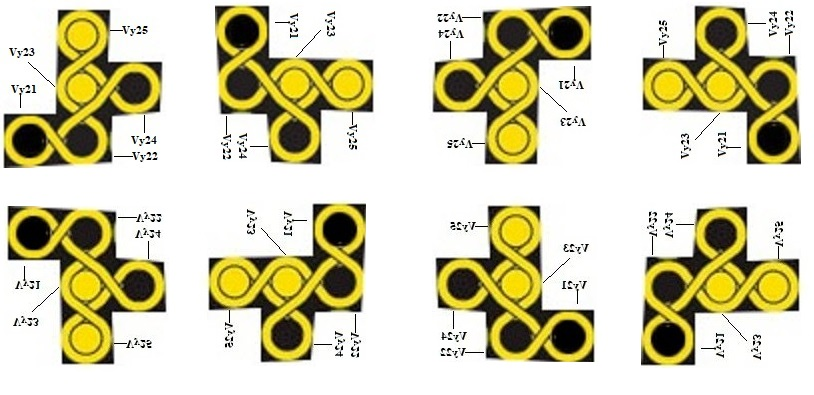
\includegraphics[scale=0.5]{domainexplain.jpg}\\
example of 8 situations
\end{center}
\circled{3} piece Yellow1
\begin{align*}
\Con{y11}{y12}{y13}=\{&((a,b),(c,d),(e,f))\in \Domain{y11}\times \Domain{y12}\times\Domain{y13}\mid\\
&(c = a + 1,\hspace{1ex}d = b,\hspace{1ex}e = a + 2, \hspace{1ex}f = b)\hspace{1ex} or\\
&(c = a,\hspace{1ex}d = b+1,\hspace{1ex}e = a, \hspace{1ex}f = b+2)\hspace{1ex} or\\
&(c = a-1,\hspace{1ex}d = b,\hspace{1ex}e = a-2,\hspace{1ex} f = b)\hspace{1ex} or\\
&(c = a,\hspace{1ex}d = b-1,\hspace{1ex}e = a, \hspace{1ex}f = b-2)\hspace{3ex} \}
\end{align*} 
\\\circled{4} piece Yellow2
\begin{align*}
\Cons{y21}{y22}{y23}{y24}{y25}=\{&((a,b),(c,d),(e,f),(g,h),(i,j))\in \\
&\Domain {y21} \times \Domain{y22}\times \Domain{y23}\times \Domain{y24}\times \Domain{y25} \mid\\
&(c = a + 1,\hspace{1ex}d = b,\hspace{1ex}e=a+1,\hspace{1ex}f=b+1,
\\&g=a+2,\hspace{1ex}h=b+1,\hspace{1ex}i=a+1,\hspace{1ex}j=b+2)\hspace{1ex} or \\
&(c = a ,\hspace{1ex}d = b+1,\hspace{1ex}e=a-1,\hspace{1ex}f=b+1,
\\&g=a-1,\hspace{1ex}h=b+2,\hspace{1ex}i=a-2,\hspace{1ex}j=b+1)\hspace{1ex} or \\
&(c = a-1 ,\hspace{1ex}d = b,\hspace{1ex}e=a-1,\hspace{1ex}f=b-1,
\\&g=a-2,\hspace{1ex}h=b-1,\hspace{1ex}i=a-1,\hspace{1ex}j=b-2)\hspace{1ex} or \\
&(c = a ,\hspace{1ex}d = b-1,\hspace{1ex}e=a+1,\hspace{1ex}f=b-1,
\\&g=a+1,\hspace{1ex}h=b-2,\hspace{1ex}i=a+2,\hspace{1ex}j=b-1)\hspace{1ex} or \\
&(c = a-1 ,\hspace{1ex}d = b,\hspace{1ex}e=a-1,\hspace{1ex}f=b+1,
\\&g=a-2,\hspace{1ex}h=b+1,\hspace{1ex}i=a-1,\hspace{1ex}j=b+2)\hspace{1ex} or \\
&(c = a ,\hspace{1ex}d = b-1,\hspace{1ex}e=a-1,\hspace{1ex}f=b-1,
\\&g=a-1,\hspace{1ex}h=b-2,\hspace{1ex}i=a-2,\hspace{1ex}j=b-1)\hspace{1ex} or \\
&(c = a+1 ,\hspace{1ex}d = b,\hspace{1ex}e=a+1,\hspace{1ex}f=b-1,
\\&g=a+2,\hspace{1ex}h=b-1,\hspace{1ex}i=a+1,\hspace{1ex}j=b-2)\hspace{1ex} or \\
&(c = a ,\hspace{1ex}d = b+1,\hspace{1ex}e=a+1,\hspace{1ex}f=b+1,
\\&g=a+1,\hspace{1ex}h=b+2,\hspace{1ex}i=a+2,\hspace{1ex}j=b+1)\hspace{3ex}\}
\end{align*}  
\\\circled{5} piece Blue1 
\begin{align*}
\Cons{b11}{b12}{b13}{b14}{b15}=\{&((a,b),(c,d),(e,f),(g,h),(i,j))\in \\
&\Domain {b11} \times \Domain{b12}\times \Domain{b13}\times \Domain{b14}\times \Domain{b15} \mid\\
&(c = a,\hspace{1ex}d = b+1,\hspace{1ex}e=a+1,\hspace{1ex}f=b+1,
\\&g=a,\hspace{1ex}h=b+2,\hspace{1ex}i=a+1,\hspace{1ex}j=b+2)\hspace{1ex} or \\
&(c = a-1 ,\hspace{1ex}d = b,\hspace{1ex}e=a-1,\hspace{1ex}f=b+1,
\\&g=a-2,\hspace{1ex}h=b,\hspace{1ex}i=a-2,\hspace{1ex}j=b+1)\hspace{1ex} or \\
&(c = a ,\hspace{1ex}d = b-1,\hspace{1ex}e=a-1,\hspace{1ex}f=b-1,
\\&g=a,\hspace{1ex}h=b-2,\hspace{1ex}i=a-1,\hspace{1ex}j=b-2)\hspace{1ex} or \\
&(c = a+1 ,\hspace{1ex}d = b,\hspace{1ex}e=a+1,\hspace{1ex}f=b-1,
\\&g=a+2,\hspace{1ex}h=b,\hspace{1ex}i=a+2,\hspace{1ex}j=b-1)\hspace{1ex} or \\
&(c = a,\hspace{1ex}d = b+1,\hspace{1ex}e=a-1,\hspace{1ex}f=b+1,
\\&g=a,\hspace{1ex}h=b+2,\hspace{1ex}i=a-1,\hspace{1ex}j=b+2)\hspace{1ex} or \\
&(c = a-1 ,\hspace{1ex}d = b,\hspace{1ex}e=a-1,\hspace{1ex}f=b-1,
\\&g=a-2,\hspace{1ex}h=b,\hspace{1ex}i=a-2,\hspace{1ex}j=b-1)\hspace{1ex} or \\
&(c = a ,\hspace{1ex}d = b-1,\hspace{1ex}e=a+1,\hspace{1ex}f=b-1,
\\&g=a,\hspace{1ex}h=b-2,\hspace{1ex}i=a+1,\hspace{1ex}j=b-2)\hspace{1ex} or \\
&(c = a+1 ,\hspace{1ex}d = b,\hspace{1ex}e=a+1,\hspace{1ex}f=b+1,
\\&g=a+2,\hspace{1ex}h=b,\hspace{1ex}i=a+2,\hspace{1ex}j=b+1)\hspace{3ex}\}
\end{align*}  
\\\circled{6} piece Blue2 
\begin{align*}
\Const{b21}{b22}{b23}{b24}=\{&((a,b),(c,d),(e,f),(g,h))\in \Domain{b21}\times \Domain{b22}\times\Domain{b23}\times\Domain{b24}\mid\\
&(c = a + 1,\hspace{1ex}d = b,\hspace{1ex}e = a + 2, \hspace{1ex}f = b,\hspace{1ex}g=a+3,\hspace{1ex}h=b)\hspace{1ex} or\\
&(c = a,\hspace{1ex}d = b+1,\hspace{1ex}e = a, \hspace{1ex}f = b+2,\hspace{1ex}g=a,\hspace{1ex}h=b+3)\hspace{1ex} or\\
&(c = a-1,\hspace{1ex}d = b,\hspace{1ex}e = a-2,\hspace{1ex} f = b,\hspace{1ex}g=a-3,\hspace{1ex}h=b)\hspace{1ex} or\\
&(c = a,\hspace{1ex}d = b-1,\hspace{1ex}e = a, \hspace{1ex}f = b-2,\hspace{1ex}g=a,\hspace{1ex}h=b-3)\hspace{3ex} \}
\end{align*}
\\\circled{7} piece Green1 
\begin{align*}
\Const{g11}{g12}{g13}{g14}=\{&((a,b),(c,d),(e,f),(g,h))\in \Domain{g11}\times \Domain{g12}\times\Domain{g13}\times\Domain{g14}\mid\\
&(c = a + 1,\hspace{1ex}d = b,\hspace{1ex}e = a + 2, \hspace{1ex}f = b,\hspace{1ex}g=a+1,\hspace{1ex}h=b+1)\hspace{1ex} or\\
&(c = a,\hspace{1ex}d = b+1,\hspace{1ex}e = a, \hspace{1ex}f = b+2,\hspace{1ex}g=a-1,\hspace{1ex}h=b+1)\hspace{1ex} or\\
&(c = a-1,\hspace{1ex}d = b,\hspace{1ex}e = a-2,\hspace{1ex} f = b,\hspace{1ex}g=a-1,\hspace{1ex}h=b-1)\hspace{1ex} or\\
&(c = a,\hspace{1ex}d = b-1,\hspace{1ex}e = a, \hspace{1ex}f = b-2,\hspace{1ex}g=a+1,\hspace{1ex}h=b-1)\hspace{1ex} or\\
&(c = a-1,\hspace{1ex}d = b,\hspace{1ex}e = a-2, \hspace{1ex}f = b,\hspace{1ex}g=a-1,\hspace{1ex}h=b-1)\hspace{1ex} or\\
&(c = a,\hspace{1ex}d = b-1,\hspace{1ex}e = a, \hspace{1ex}f = b-2,\hspace{1ex}g=a-1,\hspace{1ex}h=b-1)\hspace{1ex} or\\
&(c = a+1,\hspace{1ex}d = b,\hspace{1ex}e = a+2, \hspace{1ex}f = b,\hspace{1ex}g=a+1,\hspace{1ex}h=b-1)\hspace{1ex} or\\
&(c = a,\hspace{1ex}d = b+1,\hspace{1ex}e = a, \hspace{1ex}f = b+2,\hspace{1ex}g=a+1,\hspace{1ex}h=b+1)\hspace{3ex} \}
\end{align*}
\\\circled{8} piece Green2 
\begin{align*}
\Con{g21}{g22}{g23}=\{&((a,b),(c,d),(e,f))\in \Domain{g21}\times \Domain{g22}\times\Domain{g23}\mid\\
&(c = a+1,\hspace{1ex}d = b,\hspace{1ex}e = a+1, \hspace{1ex}f = b+1)\hspace{1ex} or\\
&(c = a,\hspace{1ex}d = b+1,\hspace{1ex}e = a-1, \hspace{1ex}f = b+1)\hspace{1ex} or\\
&(c = a-1,\hspace{1ex}d = b,\hspace{1ex}e = a-1,\hspace{1ex} f = b-1)\hspace{1ex} or\\
&(c = a,\hspace{1ex}d = b-1,\hspace{1ex}e = a+1, \hspace{1ex}f = b-1)\hspace{1ex} or\\
&(c = a-1,\hspace{1ex}d = b,\hspace{1ex}e = a-1, \hspace{1ex}f = b+1)\hspace{1ex} or\\
&(c = a,\hspace{1ex}d = b-1,\hspace{1ex}e = a-1, \hspace{1ex}f = b-1)\hspace{1ex} or\\
&(c = a+1,\hspace{1ex}d = b,\hspace{1ex}e = a+1, \hspace{1ex}f = b-1)\hspace{1ex} or\\
&(c = a,\hspace{1ex}d = b+1,\hspace{1ex}e = a+1, \hspace{1ex}f = b+1) \hspace{3ex} \}
\end{align*}
\\\circled{9} piece Red1 
\begin{align*}
\Const{r11}{r12}{r13}{r14}=\{&((a,b),(c,d),(e,f),(g,h))\in \Domain{r11}\times \Domain{r12}\times\Domain{r13}\times\Domain{r14}\mid\\
&(c = a + 1,\hspace{1ex}d = b,\hspace{1ex}e = a + 1, \hspace{1ex}f = b+1,\hspace{1ex}g=a+2,\hspace{1ex}h=b+1)\hspace{1ex} or\\
&(c = a,\hspace{1ex}d = b+1,\hspace{1ex}e = a-1, \hspace{1ex}f = b+1,\hspace{1ex}g=a-1,\hspace{1ex}h=b+2)\hspace{1ex} or\\
&(c = a-1,\hspace{1ex}d = b,\hspace{1ex}e = a-1,\hspace{1ex} f = b-1,\hspace{1ex}g=a-2,\hspace{1ex}h=b-1)\hspace{1ex} or\\
&(c = a,\hspace{1ex}d = b-1,\hspace{1ex}e = a+1, \hspace{1ex}f = b-1,\hspace{1ex}g=a+1,\hspace{1ex}h=b-2)\hspace{1ex} or\\
&(c = a-1,\hspace{1ex}d = b,\hspace{1ex}e = a-1, \hspace{1ex}f = b+1,\hspace{1ex}g=a-2,\hspace{1ex}h=b+1)\hspace{1ex} or\\
&(c = a,\hspace{1ex}d = b-1,\hspace{1ex}e = a-1, \hspace{1ex}f = b-1,\hspace{1ex}g=a-1,\hspace{1ex}h=b-2)\hspace{1ex} or\\
&(c = a+1,\hspace{1ex}d = b,\hspace{1ex}e = a+1, \hspace{1ex}f = b-1,\hspace{1ex}g=a+2,\hspace{1ex}h=b-1)\hspace{1ex} or\\
&(c = a,\hspace{1ex}d = b+1,\hspace{1ex}e = a+1, \hspace{1ex}f = b+1,\hspace{1ex}g=a+1,\hspace{1ex}h=b+2)\hspace{3ex} \} 
\end{align*}
\\\circled{10} piece Red2 
\begin{align*}
\Const{r21}{r22}{r23}{r24}=\{&((a,b),(c,d),(e,f),(g,h))\in \Domain{r21}\times \Domain{r22}\times\Domain{r23}\times\Domain{r24}\mid\\
&(c = a + 1,\hspace{1ex}d = b,\hspace{1ex}e = a + 2, \hspace{1ex}f = b,\hspace{1ex}g=a,\hspace{1ex}h=b+1)\hspace{1ex} or\\
&(c = a,\hspace{1ex}d = b+1,\hspace{1ex}e = a, \hspace{1ex}f = b+2,\hspace{1ex}g=a-1,\hspace{1ex}h=b)\hspace{1ex} or\\
&(c = a-1,\hspace{1ex}d = b,\hspace{1ex}e = a-2,\hspace{1ex} f = b,\hspace{1ex}g=a,\hspace{1ex}h=b-1)\hspace{1ex} or\\
&(c = a,\hspace{1ex}d = b-1,\hspace{1ex}e = a, \hspace{1ex}f = b-2,\hspace{1ex}g=a+1,\hspace{1ex}h=b)\hspace{1ex} or\\
&(c = a-1,\hspace{1ex}d = b,\hspace{1ex}e = a-2, \hspace{1ex}f = b,\hspace{1ex}g=a,\hspace{1ex}h=b+1)\hspace{1ex} or\\
&(c = a,\hspace{1ex}d = b-1,\hspace{1ex}e = a, \hspace{1ex}f = b-2,\hspace{1ex}g=a-1,\hspace{1ex}h=b)\hspace{1ex} or\\
&(c = a+1,\hspace{1ex}d = b,\hspace{1ex}e = a+2, \hspace{1ex}f = b,\hspace{1ex}g=a,\hspace{1ex}h=b-1)\hspace{1ex} or\\
&(c = a,\hspace{1ex}d = b+1,\hspace{1ex}e = a, \hspace{1ex}f = b+2,\hspace{1ex}g=a+1,\hspace{1ex}h=b)\hspace{3ex} \} 
\end{align*}
\\\circled{11} Yellow peg1
\begin{align*}  
\Constraint{py1} = &\{((a,b),(c,d))\in \Domain{py1} \times \Domain{y11}\mid c = a \hspace{1ex} , \hspace{1ex}  d = b\}\hspace{1ex} \cup  
\\&\{((a,b),(c,d))\in \Domain{py1} \times \Domain{y21}\mid c = a \hspace{1ex} , \hspace{1ex}  d = b\}\hspace{1ex} \cup 
\\&\{ ((a,b),(c,d))\in \Domain{py1} \times \Domain{y22}\mid c = a \hspace{1ex} , \hspace{1ex}  d = b\}\hspace{1ex}\cup 
\\& \{((a,b),(c,d))\in \Domain{py1} \times \Domain{y24}\mid c = a \hspace{1ex} , \hspace{1ex}  d = b\} \hspace{1ex}\cup
\\& \{(0,0)\}
\end{align*}
\circled{12} Yellow peg2 
\begin{align*}
\Constraint{py2} = &\{((a,b),(c,d))\in \Domain{py2} \times \Domain{y11}\mid c = a \hspace{1ex} , \hspace{1ex}  d = b\} \hspace{1ex} \cup 
\\& \{((a,b),(c,d))\in \Domain{py2} \times \Domain{y21}\mid c = a \hspace{1ex} , \hspace{1ex}  d = b\} \hspace{1ex} \cup 
\\& \{ ((a,b),(c,d))\in \Domain{py2} \times \Domain{y22}\mid c = a \hspace{1ex} , \hspace{1ex}  d = b\} \hspace{1ex} \cup 
\\&\{((a,b),(c,d))\in \Domain{py2} \times \Domain{y24}\mid c = a \hspace{1ex} , \hspace{1ex}  d = b\} \hspace{1ex}\cup
\\& \{(0,0)\}
\end{align*}
\circled{13} Blue peg1 
\begin{align*}
\Constraint{pb1} = &\{((a,b),(c,d))\in \Domain{pb1} \times \Domain{b13}\mid c = a \hspace{1ex} , \hspace{1ex}  d = b\} \hspace{1ex} \cup 
\\& \{((a,b),(c,d))\in \Domain{pb1} \times \Domain{b15}\mid c = a \hspace{1ex} , \hspace{1ex}  d = b\} \hspace{1ex} \cup 
\\& \{ ((a,b),(c,d))\in \Domain{pb1} \times \Domain{b23}\mid c = a \hspace{1ex} , \hspace{1ex}  d = b\} \hspace{1ex} \cup 
\\& \{(0,0)\}
\end{align*}
\\\circled{14} Blue peg2
\begin{align*}
\Constraint{pb2} = &\{((a,b),(c,d))\in \Domain{pb2} \times \Domain{b13}\mid c = a \hspace{1ex} , \hspace{1ex}  d = b\} \hspace{1ex} \cup \\& \{((a,b),(c,d))\in \Domain{pb2} \times \Domain{b15}\mid c = a \hspace{1ex} , \hspace{1ex}  d = b\} \hspace{1ex} \cup \\& \{ ((a,b),(c,d))\in \Domain{pb2} \times \Domain{b23}\mid c = a \hspace{1ex} , \hspace{1ex}  d = b\} \hspace{1ex} \cup \\& \{(0,0)\}
\end{align*}
\circled{15} Green peg1 
\begin{align*}
\Constraint{pg1} = &\{((a,b),(c,d))\in \Domain{pg1} \times \Domain{g13}\mid c = a \hspace{1ex} , \hspace{1ex}  d = b\} \hspace{1ex} \cup 
\\& \{((a,b),(c,d))\in \Domain{pg1} \times \Domain{g14}\mid c = a \hspace{1ex} , \hspace{1ex}  d = b\} \hspace{1ex} \cup 
\\&\{ ((a,b),(c,d))\in \Domain{pg1} \times \Domain{g22}\mid c = a \hspace{1ex} , \hspace{1ex}  d = b\}\hspace{1ex} \cup 
\\&\{ ((a,b),(c,d))\in \Domain{pg1} \times \Domain{g23}\mid c = a \hspace{1ex} , \hspace{1ex}  d = b\} \hspace{1ex} \cup 
\\&\{(0,0)\}
\end{align*}
\\\circled{16} Green peg2 
\begin{align*}
\Constraint{pg2} = &\{((a,b),(c,d))\in \Domain{pg2} \times \Domain{g13}\mid c = a \hspace{1ex} , \hspace{1ex}  d = b\} \hspace{1ex} \cup 
\\&\{((a,b),(c,d))\in \Domain{pg2} \times \Domain{g14}\mid c = a \hspace{1ex} , \hspace{1ex}  d = b\} \hspace{1ex} \cup 
\\&\{ ((a,b),(c,d))\in \Domain{pg2} \times \Domain{g22}\mid c = a \hspace{1ex} , \hspace{1ex}  d = b\}\hspace{1ex} \cup 
\\&\{ ((a,b),(c,d))\in \Domain{pg2} \times \Domain{g23}\mid c = a \hspace{1ex} , \hspace{1ex}  d = b\} \hspace{1ex} \cup 
\\&\{(0,0)\}
\end{align*}
\\\circled{17} Red peg 
\begin{align*}
\Constraint{pr} = &\{((a,b),(c,d))\in \Domain{pr} \times \Domain{r12}\mid c = a \hspace{1ex} , \hspace{1ex}  d = b\} \hspace{1ex} \cup 
\\&\{((a,b),(c,d))\in \Domain{pr} \times \Domain{r21}\mid c = a \hspace{1ex} , \hspace{1ex}  d = b\} \hspace{1ex} \cup 
\\&\{ ((a,b),(c,d))\in \Domain{pr} \times \Domain{r23}\mid c = a \hspace{1ex} , \hspace{1ex}  d = b\}\hspace{1ex} \cup 
\\& \{(0,0)\}
\end{align*}

